\section{Linear Models for Classification}
\noindent
{\color{LightRubineRed} \rule{\linewidth}{1mm} }
%%%%%%%%%%%%%%
\subsection{Linear Models Revisited}
\begin{center}
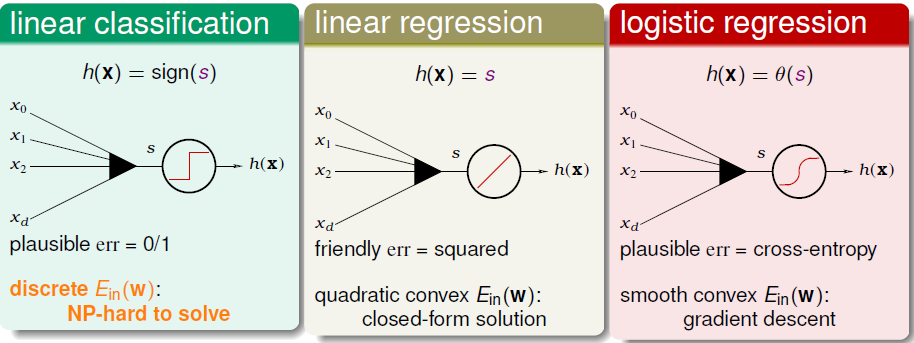
\includegraphics[width=14cm, height=5cm]{lecture11_1}\\
\end{center}
\textbf{Error Functions Revisited} \par
(ys)表示了一定的物理意义。 
\begin{center}
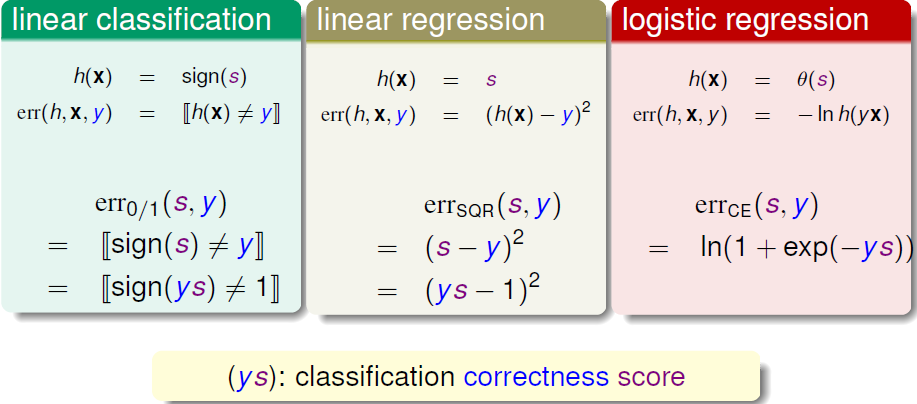
\includegraphics[width=14cm, height=6cm]{lecture11_2}\\
\end{center}
\begin{center}
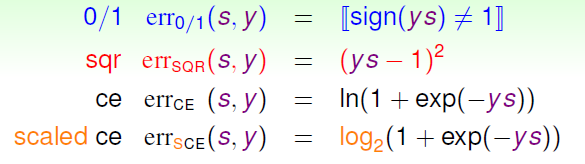
\includegraphics[width=10cm, height=3.5cm]{lecture11_3}\\
\end{center}
\begin{center}
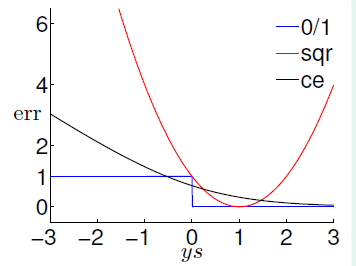
\includegraphics[width=8cm, height=6cm]{lecture11_4}\\
\end{center}
%%%%%%%%%%%%%%%%
\subsection{Stochastic Gradient Decent}
\begin{align*}
w_{t+1} \gets w_t + \eta \frac{1}{N}\sum_{n=1}\nabla_i
\end{align*}
N的数据量实在太大,我们可以使用随机抽样的方式进行。SGD = GD + zero-mean 'noise' 。用随机梯度代替真实梯度,迭代足够step后,平均随机梯度趋近于平均真是梯度。这样做简单,计算量小,适合大数据,online learning,SGD全靠抖,不是特别稳定比较GD而言。 \par

\begin{align*}
w_{t+1} \gets w_t + \eta\nabla_i
\end{align*}
SGD算法很像PLA \par
\begin{center}
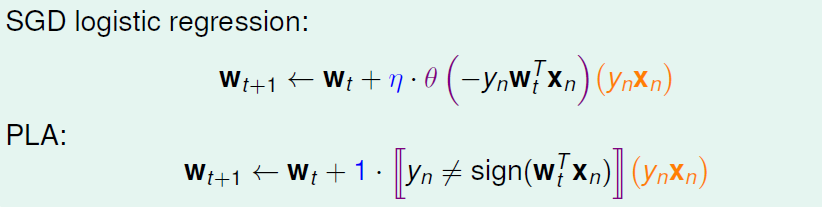
\includegraphics[width=8cm, height=2.5cm]{lecture11_5}\\
\end{center}

\subsection{Multiclass via Binary}
\begin{itemize}
	\item One vs. All [One class at a Time]
	\item One vs. One []
\end{itemize}
\begin{center}
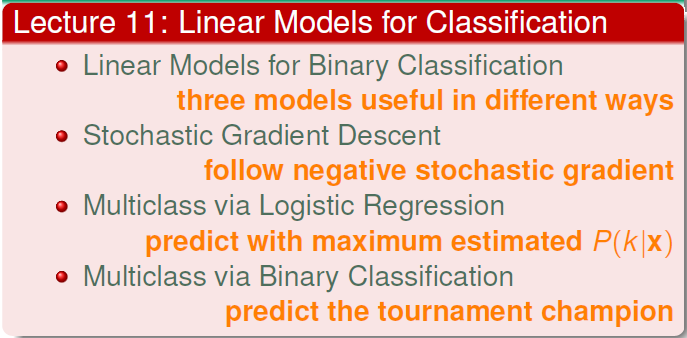
\includegraphics[width=10cm, height=5cm]{lecture11_sum}\\
\end{center}
\noindent
{\color{RubineRed} \rule{\linewidth}{1mm} }
